
\documentclass{beamer}
\usepackage{ucs}
\usepackage[utf8x]{inputenc}
\usepackage[T1]{fontenc}

\usepackage{graphicx}
\usepackage{tipa}

\begin{document}
\title{How to make the computer manage natural language choices in a language learning process? \\ Linguistic and pedagogic problems.}   
\author{Lene Antonsen, Biret Ánne Bals Baal, \\ Saara Huhmarniemi, Trond Trosterud \\ \begin{figure}  \scalebox{0.10}[0.10]{
\includegraphics{img/LogoSamisk}} \end{figure}} 
\date{} 


\frame{\titlepage} 


\frame{\frametitle{ }
\begin{block}{ }
\textit{http://giellatekno.uit.no/oahpa/}\\
\end{block}{ }
Sámi parlament and University of Tromsø have financed the work}

\frame{\frametitle{VISL-programs}
\begin{block}{ }
\textbf{For grammar learning:}\\
\end{block}{ }
Word classes, syntax
}

\frame{\frametitle{OAHPA-programs}
\begin{block}{ }
\textbf{In order to learn Sámi:}\\
\end{block}{}
\begin{itemize}
\item \textbf{Leksa}: Sátnequiz - Sámi/Norwegian and Norwegian/Sámi
\item  \textbf{Numra}: Exercise numerals
\item  \textbf{Morfa}: Exercise word inflection, also contextual
\item  \textbf{Vasta}: Exercise question anwering
\item  \textbf{Sahka}: Participate in a dialogue on a given topic
\end{itemize}
}

\frame{\frametitle{Pedagogical programs}
Pedagogical programs usually do not contain language technology, but rather
\begin{itemize}
\item multiple choice 
\item stringmatch, e.g. \textit{viesus} = 6 marks: v i e s u s
\end{itemize} \pause
\begin{block}{ }
Language technology:
\begin{itemize}
\item analysis, e.g. \textit{viesus} = \textit{viessu} N Sg Loc
\end{itemize}
\end{block}{ }
}


\frame{\frametitle{Vision} 
The program should supervise the student in the same way as a teacher does.
}

\frame{\frametitle{Vasta -- exercise question anweringe} 
\scalebox{0.90}[0.90]{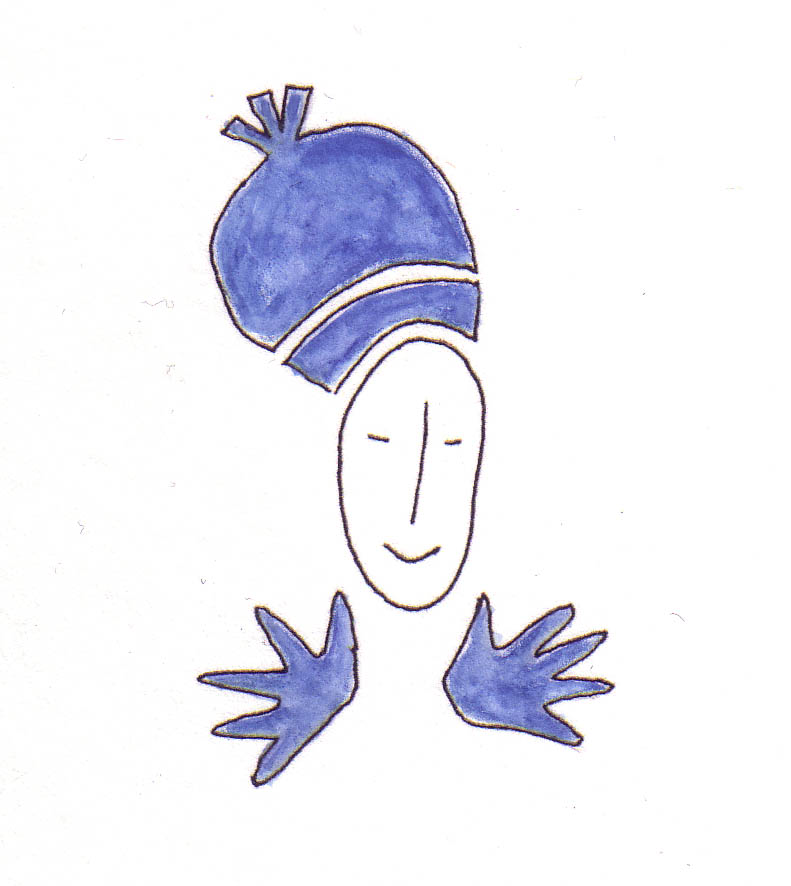
\includegraphics{img/vasta.png}} \\
}

\frame{\frametitle{Vasta} 
\scalebox{0.35}[0.35]{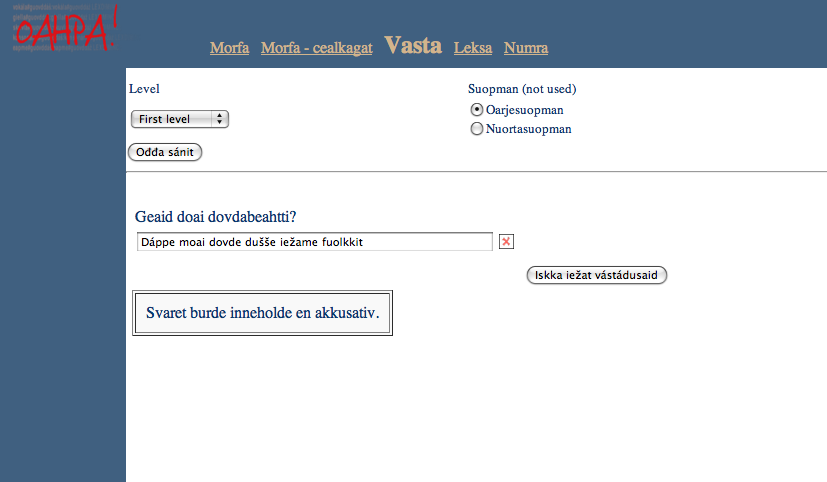
\includegraphics{img/vasta_jear.png}}
}


\frame{\frametitle{Maid don lohket ikte?} 

Acceptable answers:
\begin{itemize}
\item Mun han lohken ollu áviissaid. 
\item Ikte mun gal lohken buori girjji. 
\item In lohkan maidege. 
\item Ikte in lohkan.
\end{itemize}
}

\frame{\frametitle{Maid don lohket ikte?} 

The Vasta-program gives feedback if the answer is not acceptable:
\begin{itemize}
\item Mun lohket ollu áviissaid. \\ $\rightarrow$ Husk kongruens mellom subjekt og verbal.  
\item Mun lohken ollu áviissat. \\ $\rightarrow$ Objektet skal være i akkusativ. 
\item Don lohket ollu áviissaid. \\ $\rightarrow$ Er du sikker på at du svarer i riktig person?  
\end{itemize}
}

\frame{\frametitle{Our system} 
\scalebox{0.65}[0.65]{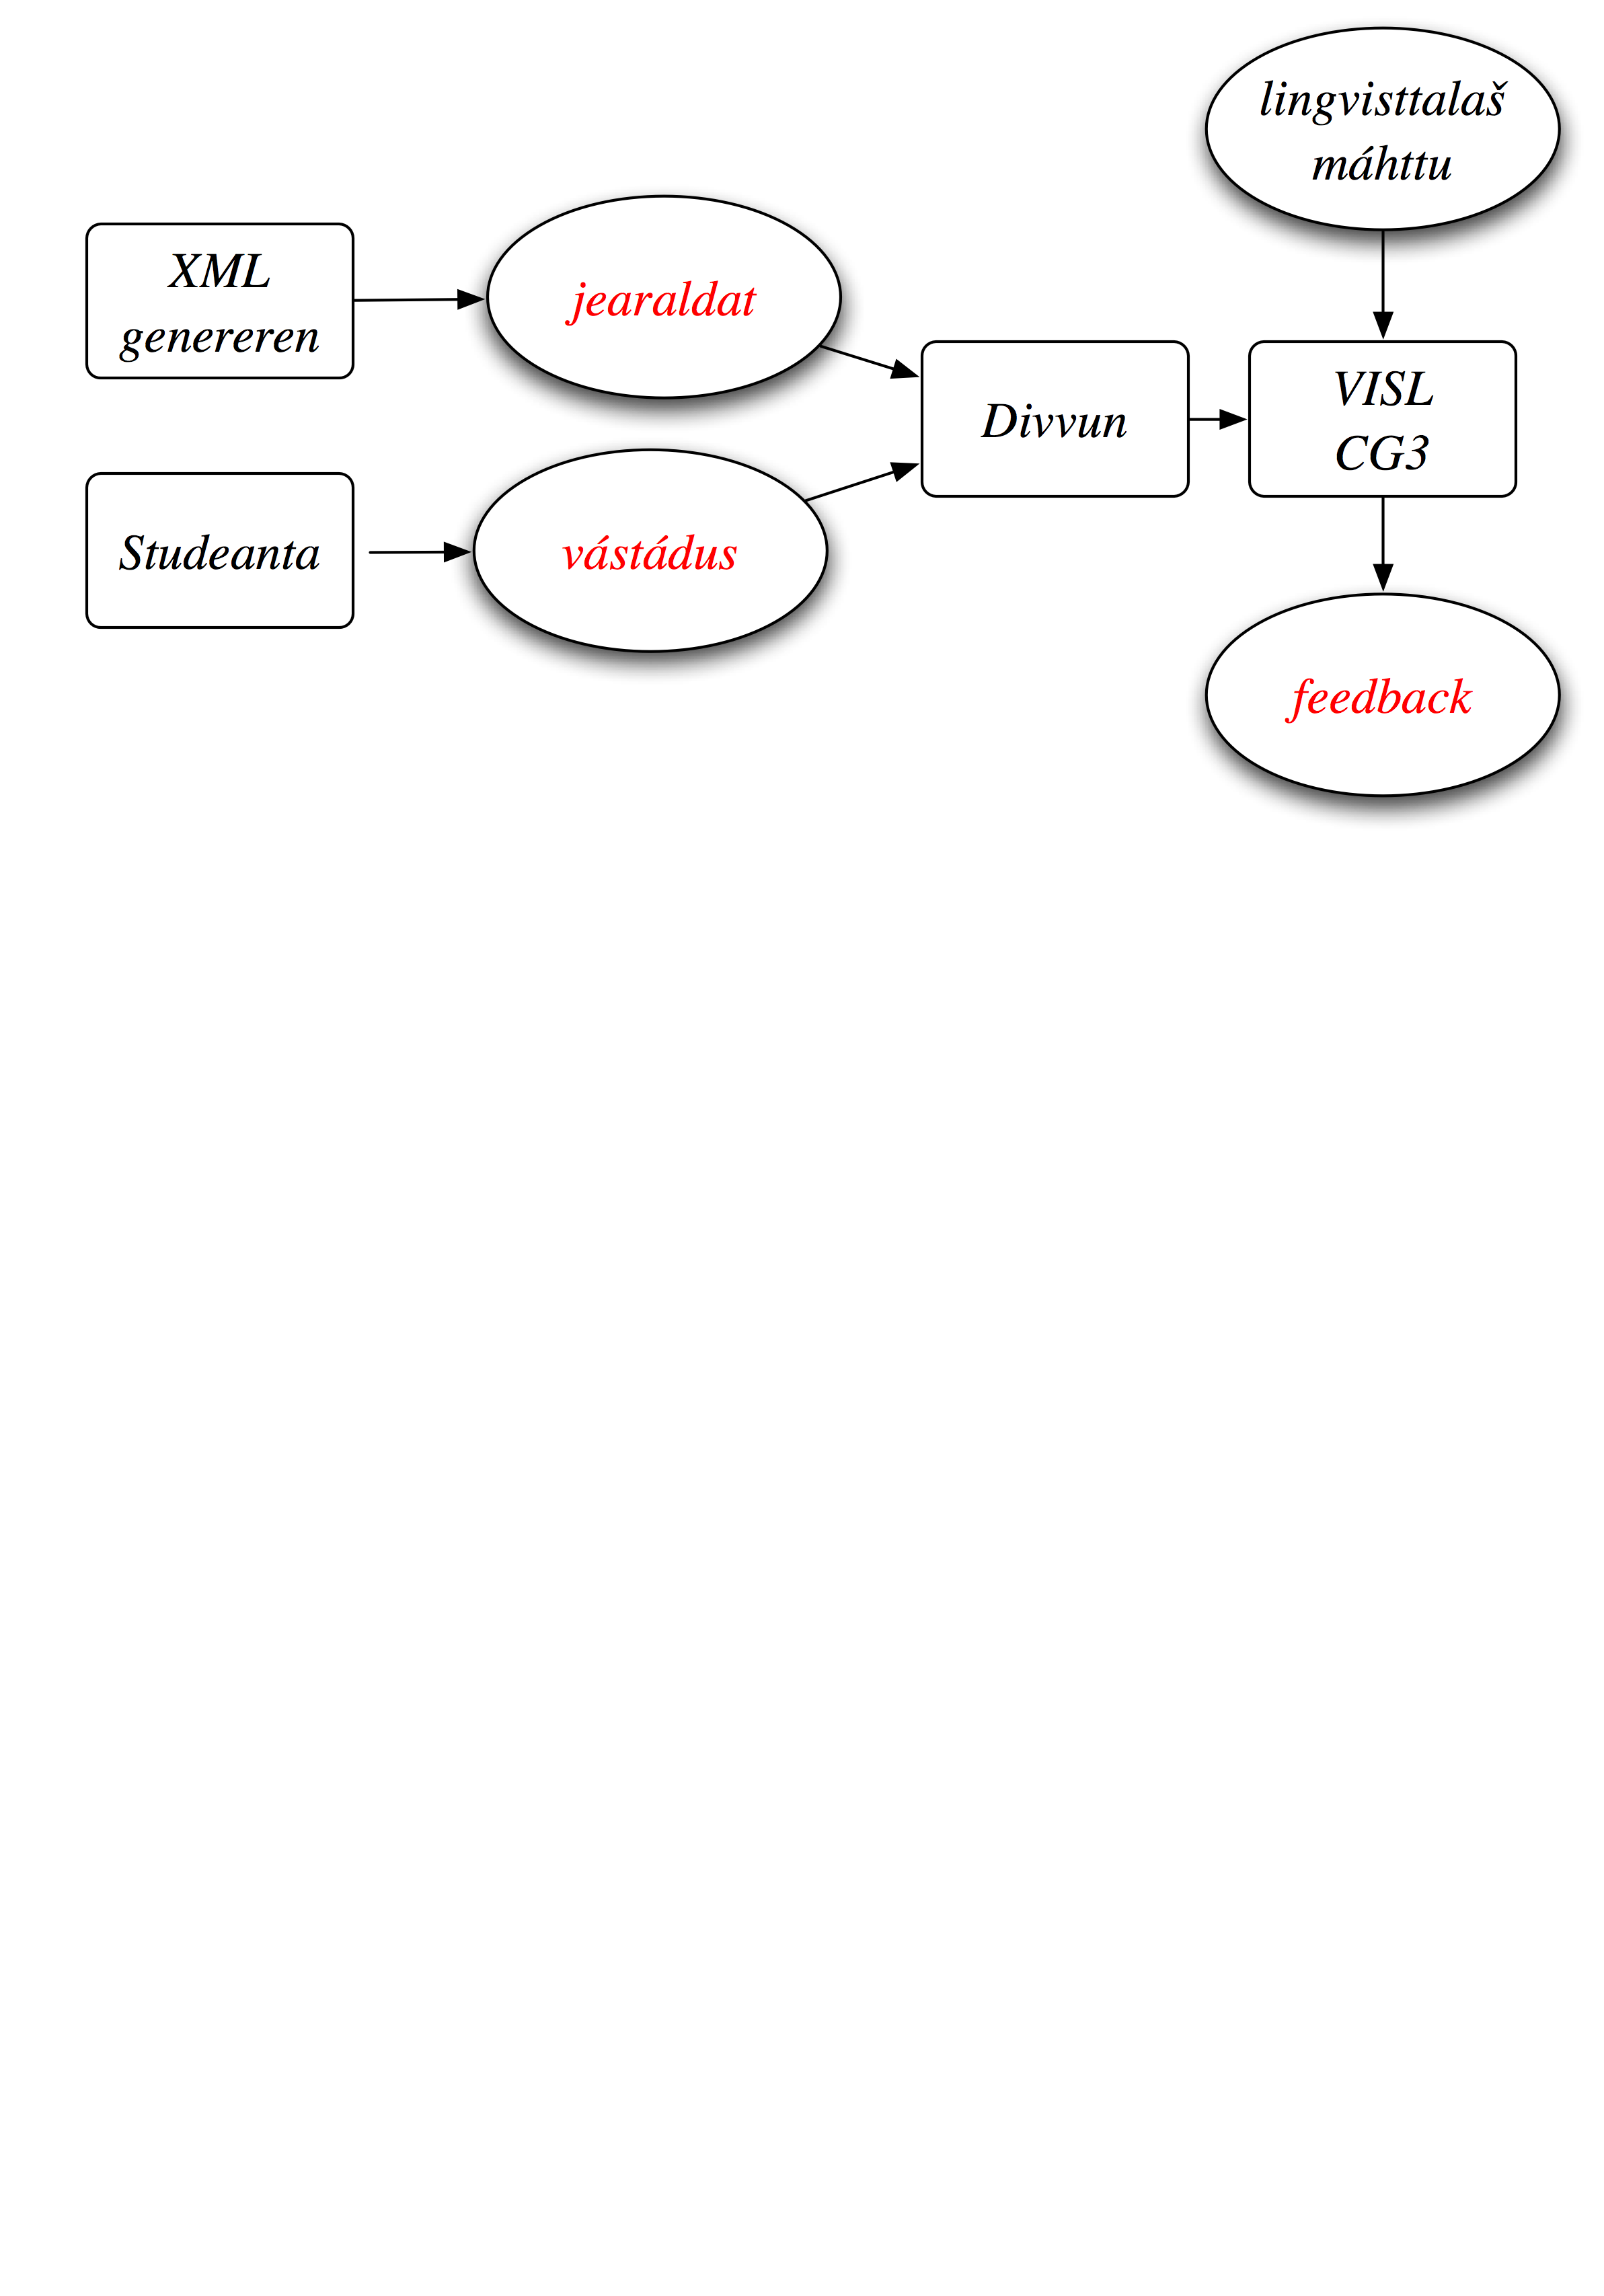
\includegraphics{img/skovi.png}} 
} 


\frame{\frametitle{Question generering} 
      <text>Maid SUBJ MAINV ikte</text>
}

\frame{\frametitle{Linguistic knowledge} 
We use our knowledge about:
\begin{itemize}
\item Sámi syntax
\item the learner´s interlanguage
\end{itemize}
}

\frame{\frametitle{Sámi syntax} 
E.g. what can be in a NP:
\begin{itemize}
\item \small{NP $\rightarrow$ Pron A N Num Adv A CC Adv A N}  \\ 	
\textit{mu boares áhku guokte hui stuora ja hirbmat váralaš beatnaga}	
\item what kind of agreement
\end{itemize}
}


\frame{\frametitle{Natural dialogue}

\begin{description}
\item [ ] D: Sidat go gáfe?   G: In diede vuos. \pause 
\item [ ] $\rightarrow$ Det er for enkelt å svare vet-ikke. Prøv igjen. \pause 
\item [ ] D: Maid háliidat borrat?   G: Láibbi. \pause 
\item [ ] $\rightarrow$ Svaret ditt må alltid inneholde et finitt verb. \pause 
\item [ ] D: Áiggut go vázzit bargui odne?   G: Ale jeara nu olu. \pause 
\item [ ] $\rightarrow$ Er du sikker på at du svarer i riktig person?
\end{description} 
}

\frame{\frametitle{Problems -- 1}
\begin{block}{ }
\textbf{Didaktihkka versus pragmatihkka} \\
\end{block}{ }
The goal is to train morphology -- Solution:
\begin{itemize}
\item{No elipsis}
\item{The finite verb is compulsatory}
\item{Answer with the same verb when it is natural to do it}
\item{No inclusive 1st person dual and plural}
\item{The answer \textit{I do not know} is not accepted}
\end{itemize}
}

\frame{\frametitle{Problems -- 2}
\begin{block}{ }
\textbf{No finite verb in the clause} \\
\end{block}{ }

\textit{*Mun vuolggan ihttin.}\\
$\rightarrow$ Svaret ditt må alltid inneholde et finitt verb. 
}

\frame{\frametitle{Problems -- 2}
\begin{block}{ }
\textbf{Possible solution:}\\
\end{block}{ }

\textit{*Mun vuolggan ihttin.}\\
$\rightarrow$ Svaret ditt må alltid inneholde et finitt verb. Kan det være en skrivefeil?
}

\frame{\frametitle{Problems -- 3}
\begin{block}{ }
\textbf{Two finite verbs in the clause} \\
\end{block}{ }
\textit{*Mun áiggun vuolggán.} versus
\textit{Mun boran haman.}\\
In a finite-finite-construction:\\ -- the verbs should have same inflection\\
-- no adverb between\\ But this is not enough
}

\frame{\frametitle{Problems -- 3}
\begin{block}{ }
\textbf{Possible solution:} \\
\end{block}{ }
Semantic set:\\
LIST INFV = \textit{astat ádjánit áigut álgit beassat berret bivvat ....} \\
\textnormal{Rule : Not possible šith (INFV finite) + (VERB finite)}
}

\frame{\frametitle{Problems -- 4}
\begin{block}{ }
\textbf{Nominative versus accusative} \\
\end{block}{ }
We cannot base our conclusion upon the word order, and the subject is not compulsory
\begin{itemize}
\item We can utilize the question - if it asks for an object (but it is still possible to answer without an object)
\end{itemize}
}

\frame{\frametitle{Problems -- 4}
\begin{block}{ }
\textbf{Possible solution:} \\
\end{block}{ }
Define the verbs and make emantic sets, e.g.: 
\begin{itemize}
\item verbs which have object as a compulsory argument (Strict Transitive Verbs)
\item verbs which cannot have a HUMAN as object \\ \pause 
\textit{borrat}   - HUMAN can be subject, not object \\
 
\textit{lohkat}  - the same, but a N Prop can be object, \\ e.g.   \textit{Ikte mun lohken Fosse.}  \\  \pause 
-- and the verb has another meaning: \textit{Mun lohken mánáid.}
\end{itemize}
}


\frame{\frametitle{Problems -- 5}
\textbf{Spelling errors} \\
\begin{enumerate}
\item the word does not exist: \\ \textit{$\rightarrow$ X finnes ikke i vårt leksikon. Kan det være en skrivefeil?}
\item unintended lemma (leksem)
\item correct lemma, but unintended word form
\end{enumerate}
}

\frame{\frametitle{Problems -- 5}
\begin{block}{ }
\textbf{We add the case suffix to the Nom} \\
\end{block}{ }
Our pedlexicon has 1512 nouns
\begin{itemize}
\item LOCATIVE -s/-is : \\
57 \% correct lemma - unintended word form (PxSg3 - e.g. \textit{viessus})  \\  0,5 \% unintended lemma \\  (e.g. \textit{eanas Adv (eatnamis)}  or \\ verb \textit{-stit} -- imperative, verbgenitive, negation -- e.g. \textit{čogus (čohkumis)} )
\end{itemize}
}

\frame{\frametitle{Problems -- 5}
\textbf{We add the case suffix to the Nom} \\
\begin{itemize}
\item LOCATIVE -s/-is: \\
57 \% correct lemma - unintended word form \\  
0,5 \% unintended lemma \\
\item ILLATIVE -i/-ii: \\
0 \% correct lemma - unintended word form \\  2,3 \% unintended lemma \\ (mostly Verb past tense Sg3, e.g. \textit{báddii (báddái)}) 
\end{itemize}
}

\frame{\frametitle{Problems -- 5a}
\begin{block}{ }
\textbf{Spelling error gives unintended inflexion} \\
\end{block}{ }
e.g. possessive suffixes \\
\textit{biilas N Sg Nom Px Sg3 versus biillas N Sg Loc} \\
\textit{*Áhčči lea biilas.}
}

\frame{\frametitle{Problems -- 5a}
\begin{block}{ }
\textbf{Possible solutions:}
\end{block}{ }
\begin{itemize}
\item Remove possessive suffixes, except from when it syntactically is quite clear that it could be.
\item Make comment to the user: \\
$\rightarrow$ Mener du lokativ? I så fall er det feil stadieveksling.
\end{itemize}
}

\frame{\frametitle{Problems -- 5b}
\begin{block}{ }
\textbf{Spelling error gives unintended lemma} \\
\end{block}{ }
\begin{itemize}
\item \textit{viessut:  viessut} Inf or \textit{viessat} Imprt \\
but the student probably meant \textit{viesut} N Pl Nom.  \pause
\item \textit{luomos}: A Attr \\
\textit{*Eadni lea luomos.} \\
$\rightarrow$ Her skulle det ikke vært attributtform. \\ \pause
\textit{Gos eadni lea?} \\ 
$\rightarrow$ Svaret burde inneholde en lokativ.
\end{itemize}
}

\frame{\frametitle{Problems -- 5b}
\begin{block}{ }
\textbf{Possible solutions:}
\end{block}{ }
\begin{itemize}
\item Remove problematic lemmas and word forms
\item Identify wordpairs and ask the user: \\ $\rightarrow$ Mener du viessu = hus? I så fall er det feil stadieveksling.
\end{itemize}
}


\frame{\frametitle{Correct or not}
\begin{block}{ }
\textbf{Better that errors slip through than not accept what is correct}
\end{block}{ }
- muhto duhtágo geavaheaddji dasa?

}

\frame{\frametitle{Evaluation and improvement}
\begin{itemize}
\item{Feedback from users}
\item{Feedback from teachers}
\item{Collect a question corpus (Vasta-Internet log}
\end{itemize}
}



\end{document}

